\section{Introduction}
In the present article, we replicate the results of Jef Huisman and Franz J. Weissing, 1999, ”Biodiversity of plankton by species oscillations and chaos”\supercite{1999:Huisman}, an attempt to resolve the ”paradox of plankton”\supercite{1961:Hutchinson} with oscillations and chaos. Using a classic resource competition model and the parameter sets used in the article, the results found could be reproduced.\\
\\
According to many mathematical models, the number of plankton species in a single medium cannot exceed the number of different ressources available\supercite{1960:Hardin,1973:Phillips,1980:Armstrong}. However it is very common to observe more species than resources in real-life conditions. This phenomenon is called the ”paradox of plankton”\supercite{1961:Hutchinson}. Using numerical simulations, Huisman \& Weissing\supercite{1999:Huisman} showed that supersaturated coexistance, where more consumer sepcies than ressource coexist through oscillations or chaos, is possible.\\
\\
In addition to replication of the numerical results of Hulsman and Weissing, we also presented new experiences inspired by other articles taking up the first one, ”Does “supersaturated coexistence” resolve the “paradox of the plankton” ?”\supercite{2008:Schippers} from Peter Schippers, Anonie M. Verschoor, Matthijs Vos \& Wolf M. Mooij, 2008 and ”Towards a solution of the plankton paradox: the importance of physiology and life history”\supercite{2008:Huisman} from Jef Huisman, Anna M. Johansson, Eelke O. Folmer \& Franz J. Weissing, 2008 that corroborate the fact that the claim of a resolution of the ”paradox of plankton” might be premature.
\section{Model}
As mentioned in the introduction, the same model of planktonic biodiversity as the original paper\supercite{1999:Huisman} was chosen :\\
 Let $N_i$ and $R_j$ respectivly be the abundances of species $i$ and ressources $j$,$i\in[\![1,n]\!]$ and $j\in[\![1,k]\!]$ with $n$ and $k$ the number of different species and ressources. The time derivatives of $N_i$ and $R_j$ are given by : \\
\begin{align}
	& \frac{dN_i}{dt}= N_i(\mu_i(R_1,...,R_k)~-~m_i)\\
	& \frac{dR_j}{dt}= D(S_j-R_j) - \sum_{i=1}^n c_{ji} \mu_i(R_1,...,R_k)N_i
\end{align}
With : 
\begin{align*}
& m_i \text{ the specific mortality rate of species $i$}\\
& D \text{ the system's turnover rate}\\
& S_j \text{ the supply concentration of ressource $j$}\\
& c_{ji} \text{ the content of ressource $j$ in species $i$}\\
& \mu_i \text{ specific growth rate of species $i$, defined using the Monod equation and Liebig's law of minimum : }
\end{align*}
\begin{align}
&\mu_i(R_1,...,R_k)~=~\min_{j\in[\![1,k]\!]}(\frac{r_iR_j}{K_{ji}+R_j})
\end{align}
With : 
\begin{align*}
&r_i \text{ the maximum growth rate of species $i$}\\
&K_{	ji} \text{ the half saturation constant for ressource $j$ of species $i$}
\end{align*}
In order to reproduce the results of Huisman \& Weissing, the differential equations were integrated using the deSolve package in R, using same parameter sets and configurations as in the paper.\\
\\
Different simulations are performed and illustrated in the paper : \\
In Figure \ref{figures:Fig2} and Figure \ref{figures:Fig1} a), b) and for the bifurcation diagram of Figure \ref{figures:Fig3}, all of the species are introduced at the same time in the simulation. In Figure \ref{figures:Fig4} and Figure \ref{figures:Fig1} c), d), the species were introduced sequentially. Huisman et al. paper \supercite{1999:Huisman} have provided the starting times of each species when needed in addition to the usual parameters.\\
\\
As Schippers et al. in their paper\supercite{2008:Schippers}, we were wondering how and why the parameter sets were chosen and if the results would remain the same for slightly different parameters. Several simulations were made in Schippers et al. paper\supercite{2008:Schippers} and Huisman et al. new paper on the same subject\supercite{2008:Huisman} to test how stable was supersaturated coexistence in parameter space. In the same spirit, news test were carried out with slightly different methods :\\We chose to focus the last simulation of the paper\supercite{1999:Huisman}, displayed on Figure 4. We choose to study the $r_i$ parameter, noted $\mu_{max}$ in the papers\supercite{2008:Schippers,2008:Huisman} but, as changing only one of the $n~~r_i$ as in thoses two articles seemed too artificial, we chose to randomly pick all of the $n~~r_i$. In a second step, thoses random parameters were kept but we also tried to introduce all of the species at once, the opposite of what could be done until now in some cases where species were introduced one after the other. 
\section{Results}
We were able to reproduce the 4 Figures of Huisman \& Weissing\supercite{1999:Huisman} illustrating a supersaturated coexistence. \\
\\
For each of them, the methods and parameters provided in the article were applied and used.\\ 
\begin{figure}[H]
\begin{center} 
 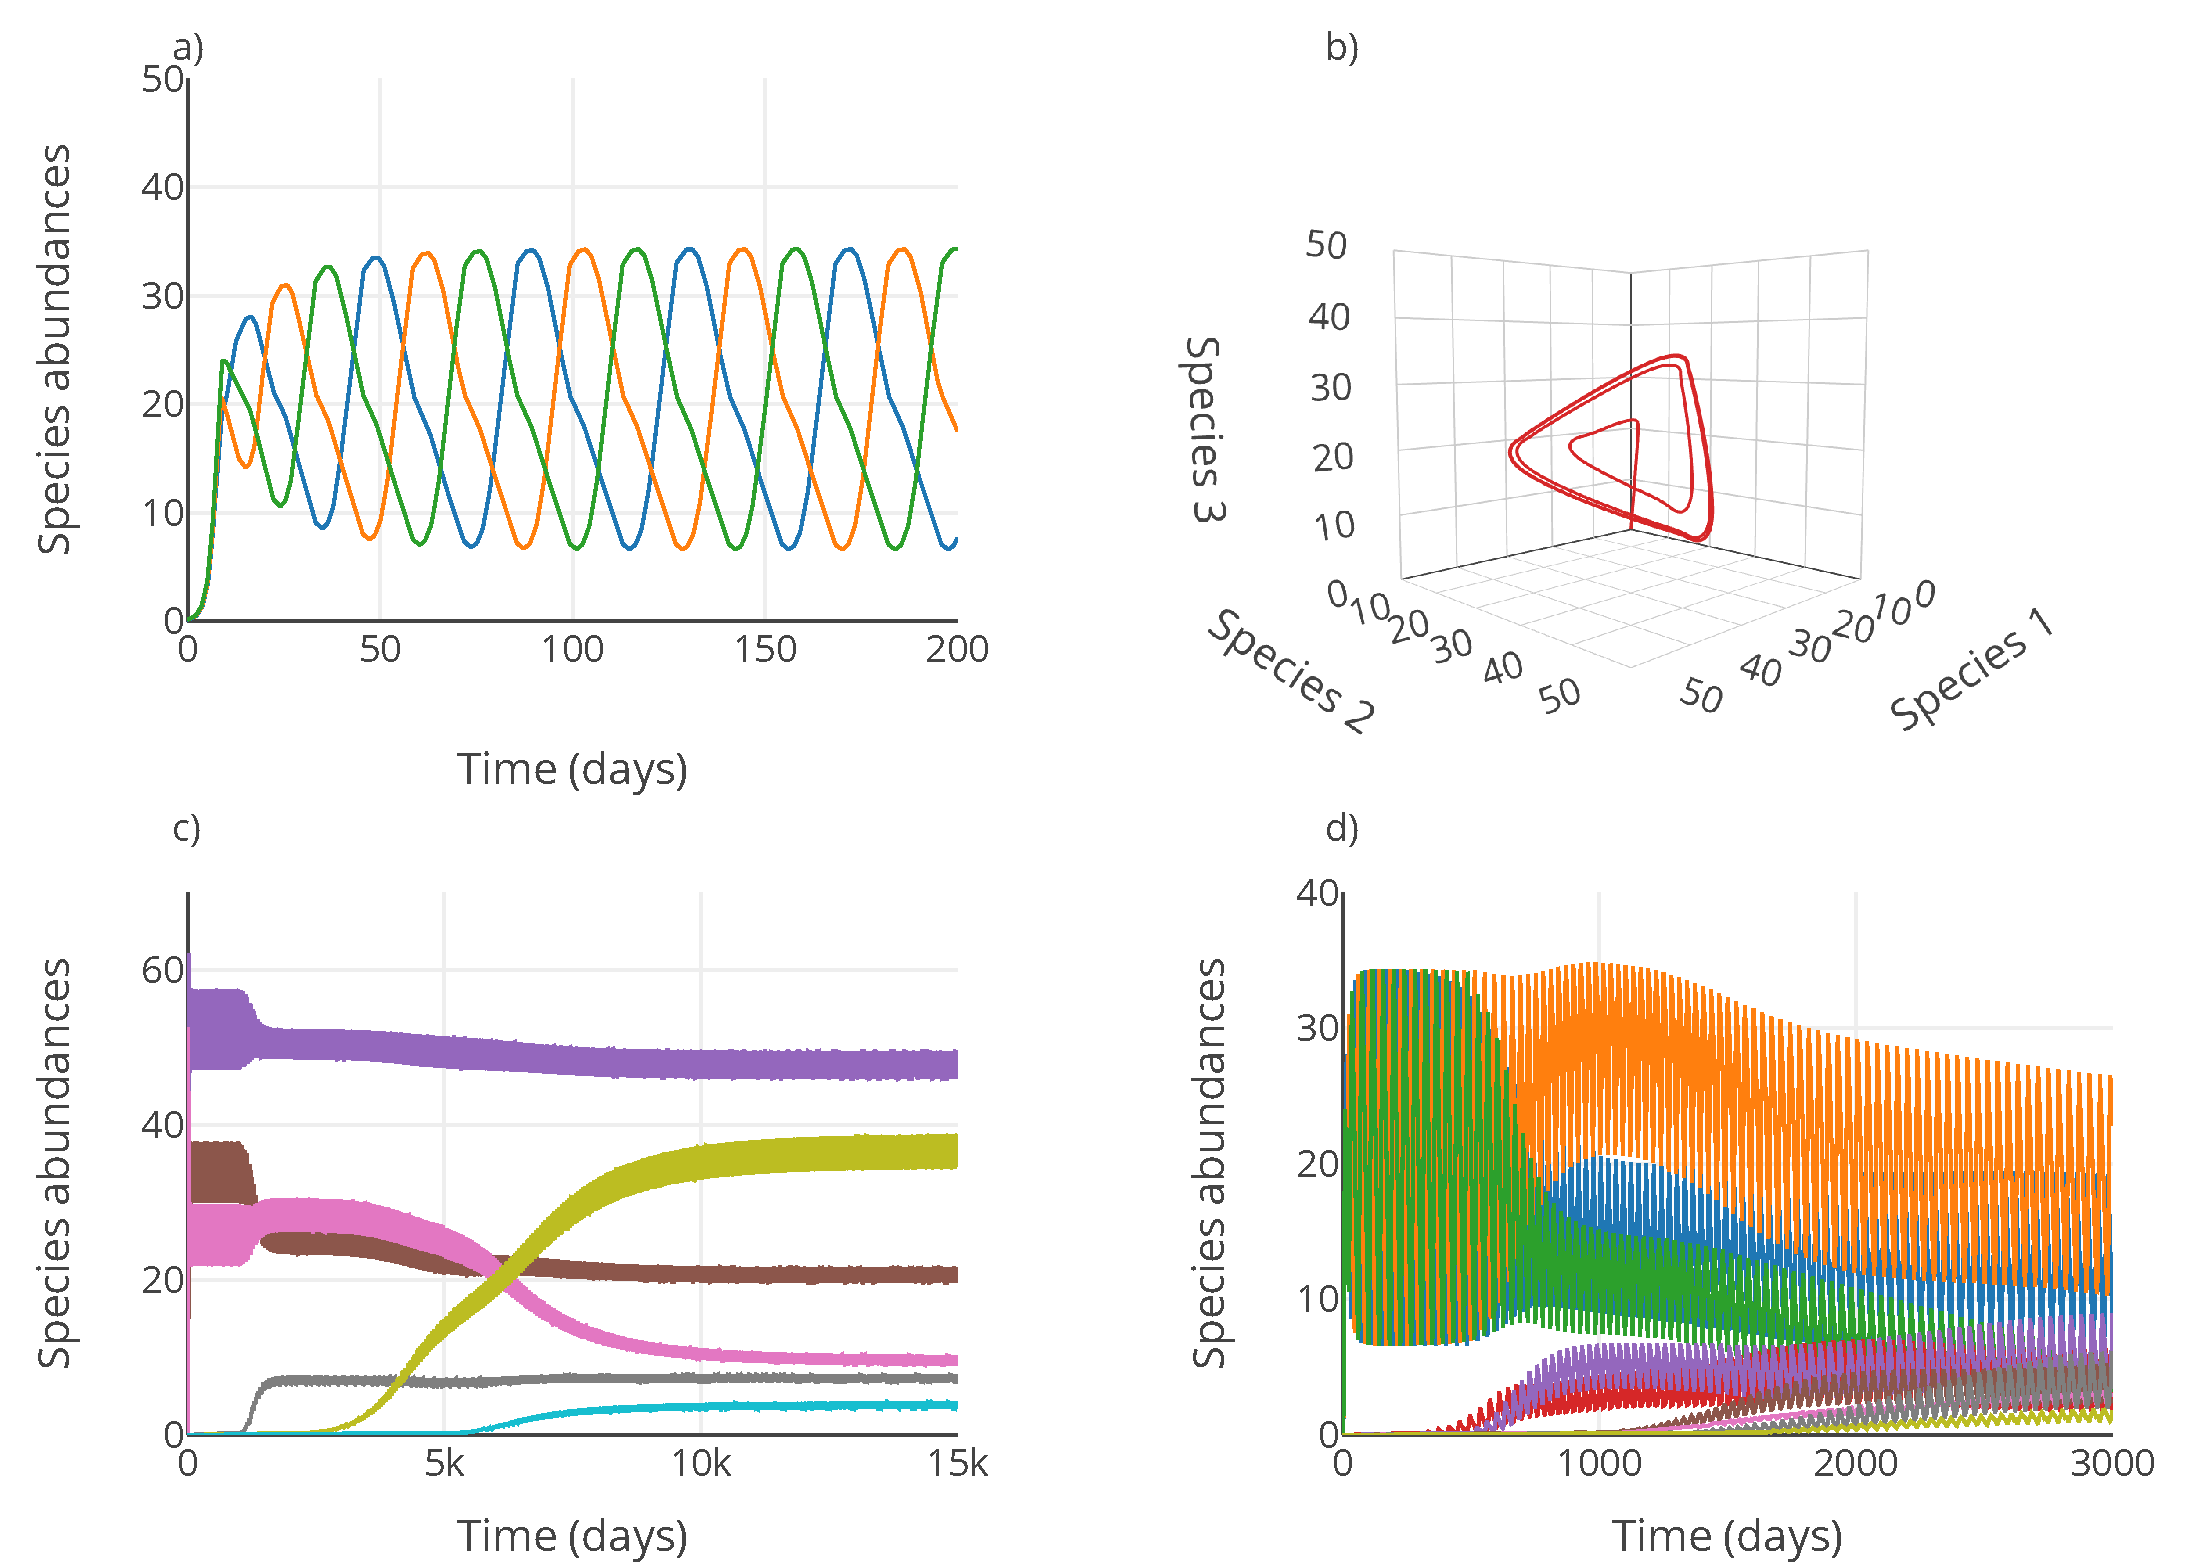
\includegraphics[width=1\textwidth]{../Code/Figures/Figure_1.pdf}
  \caption{Oscillations on three ressources. a), Time course of the abundances of three species competing for three ressources. b), The corresponding limit cycle. c), Smaill-amplitude oscillations of six species on three ressources. d),Large-amplitude oscillations of nine species on three ressources.}
  \label{figures:Fig1}
\end{center}
\end{figure}
\begin{figure}[H]
\begin{center} 
 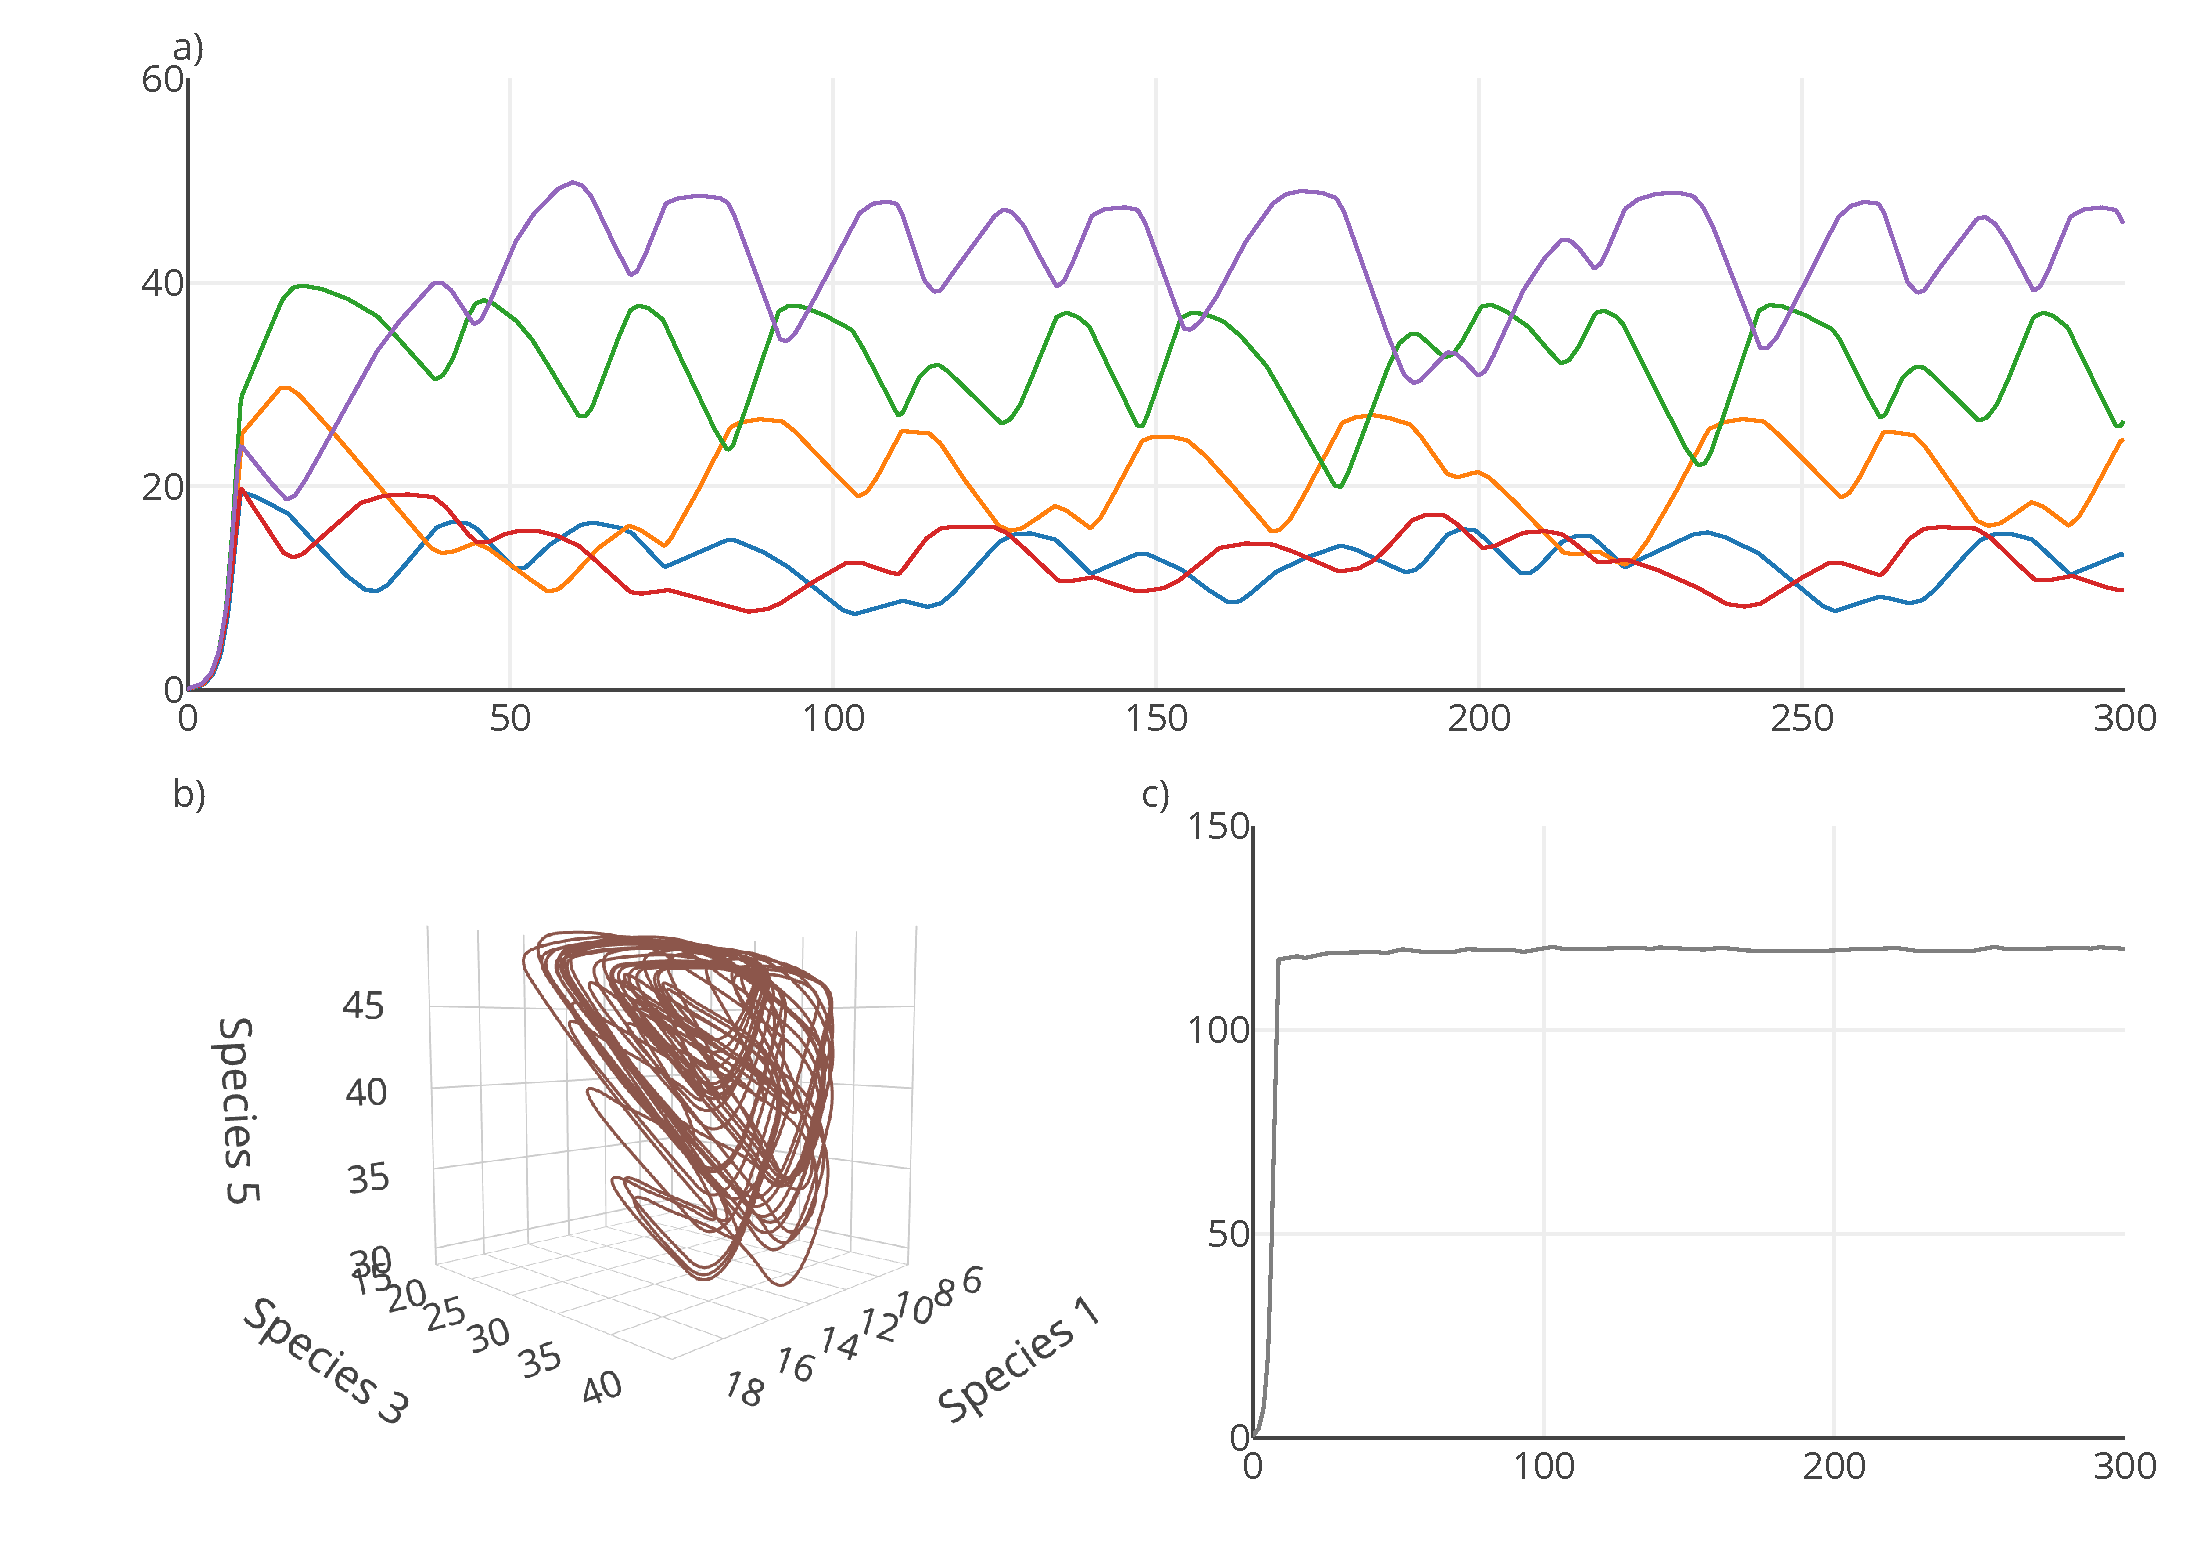
\includegraphics[width=1\textwidth]{../Code/Figures/Figure_2.pdf}
  \caption{Chaos on five ressources. a), Time course of the abundances of five species competing for five ressources. b), The corresponding chaotic attractor. The trajectory is plotted for three of the five species, from the period from $t= 1,000$ to $t=2,000$ days. c), Time course of total community biomass.}
  \label{figures:Fig2}
\end{center}
\end{figure}
\begin{figure}[H]
\begin{center} 
 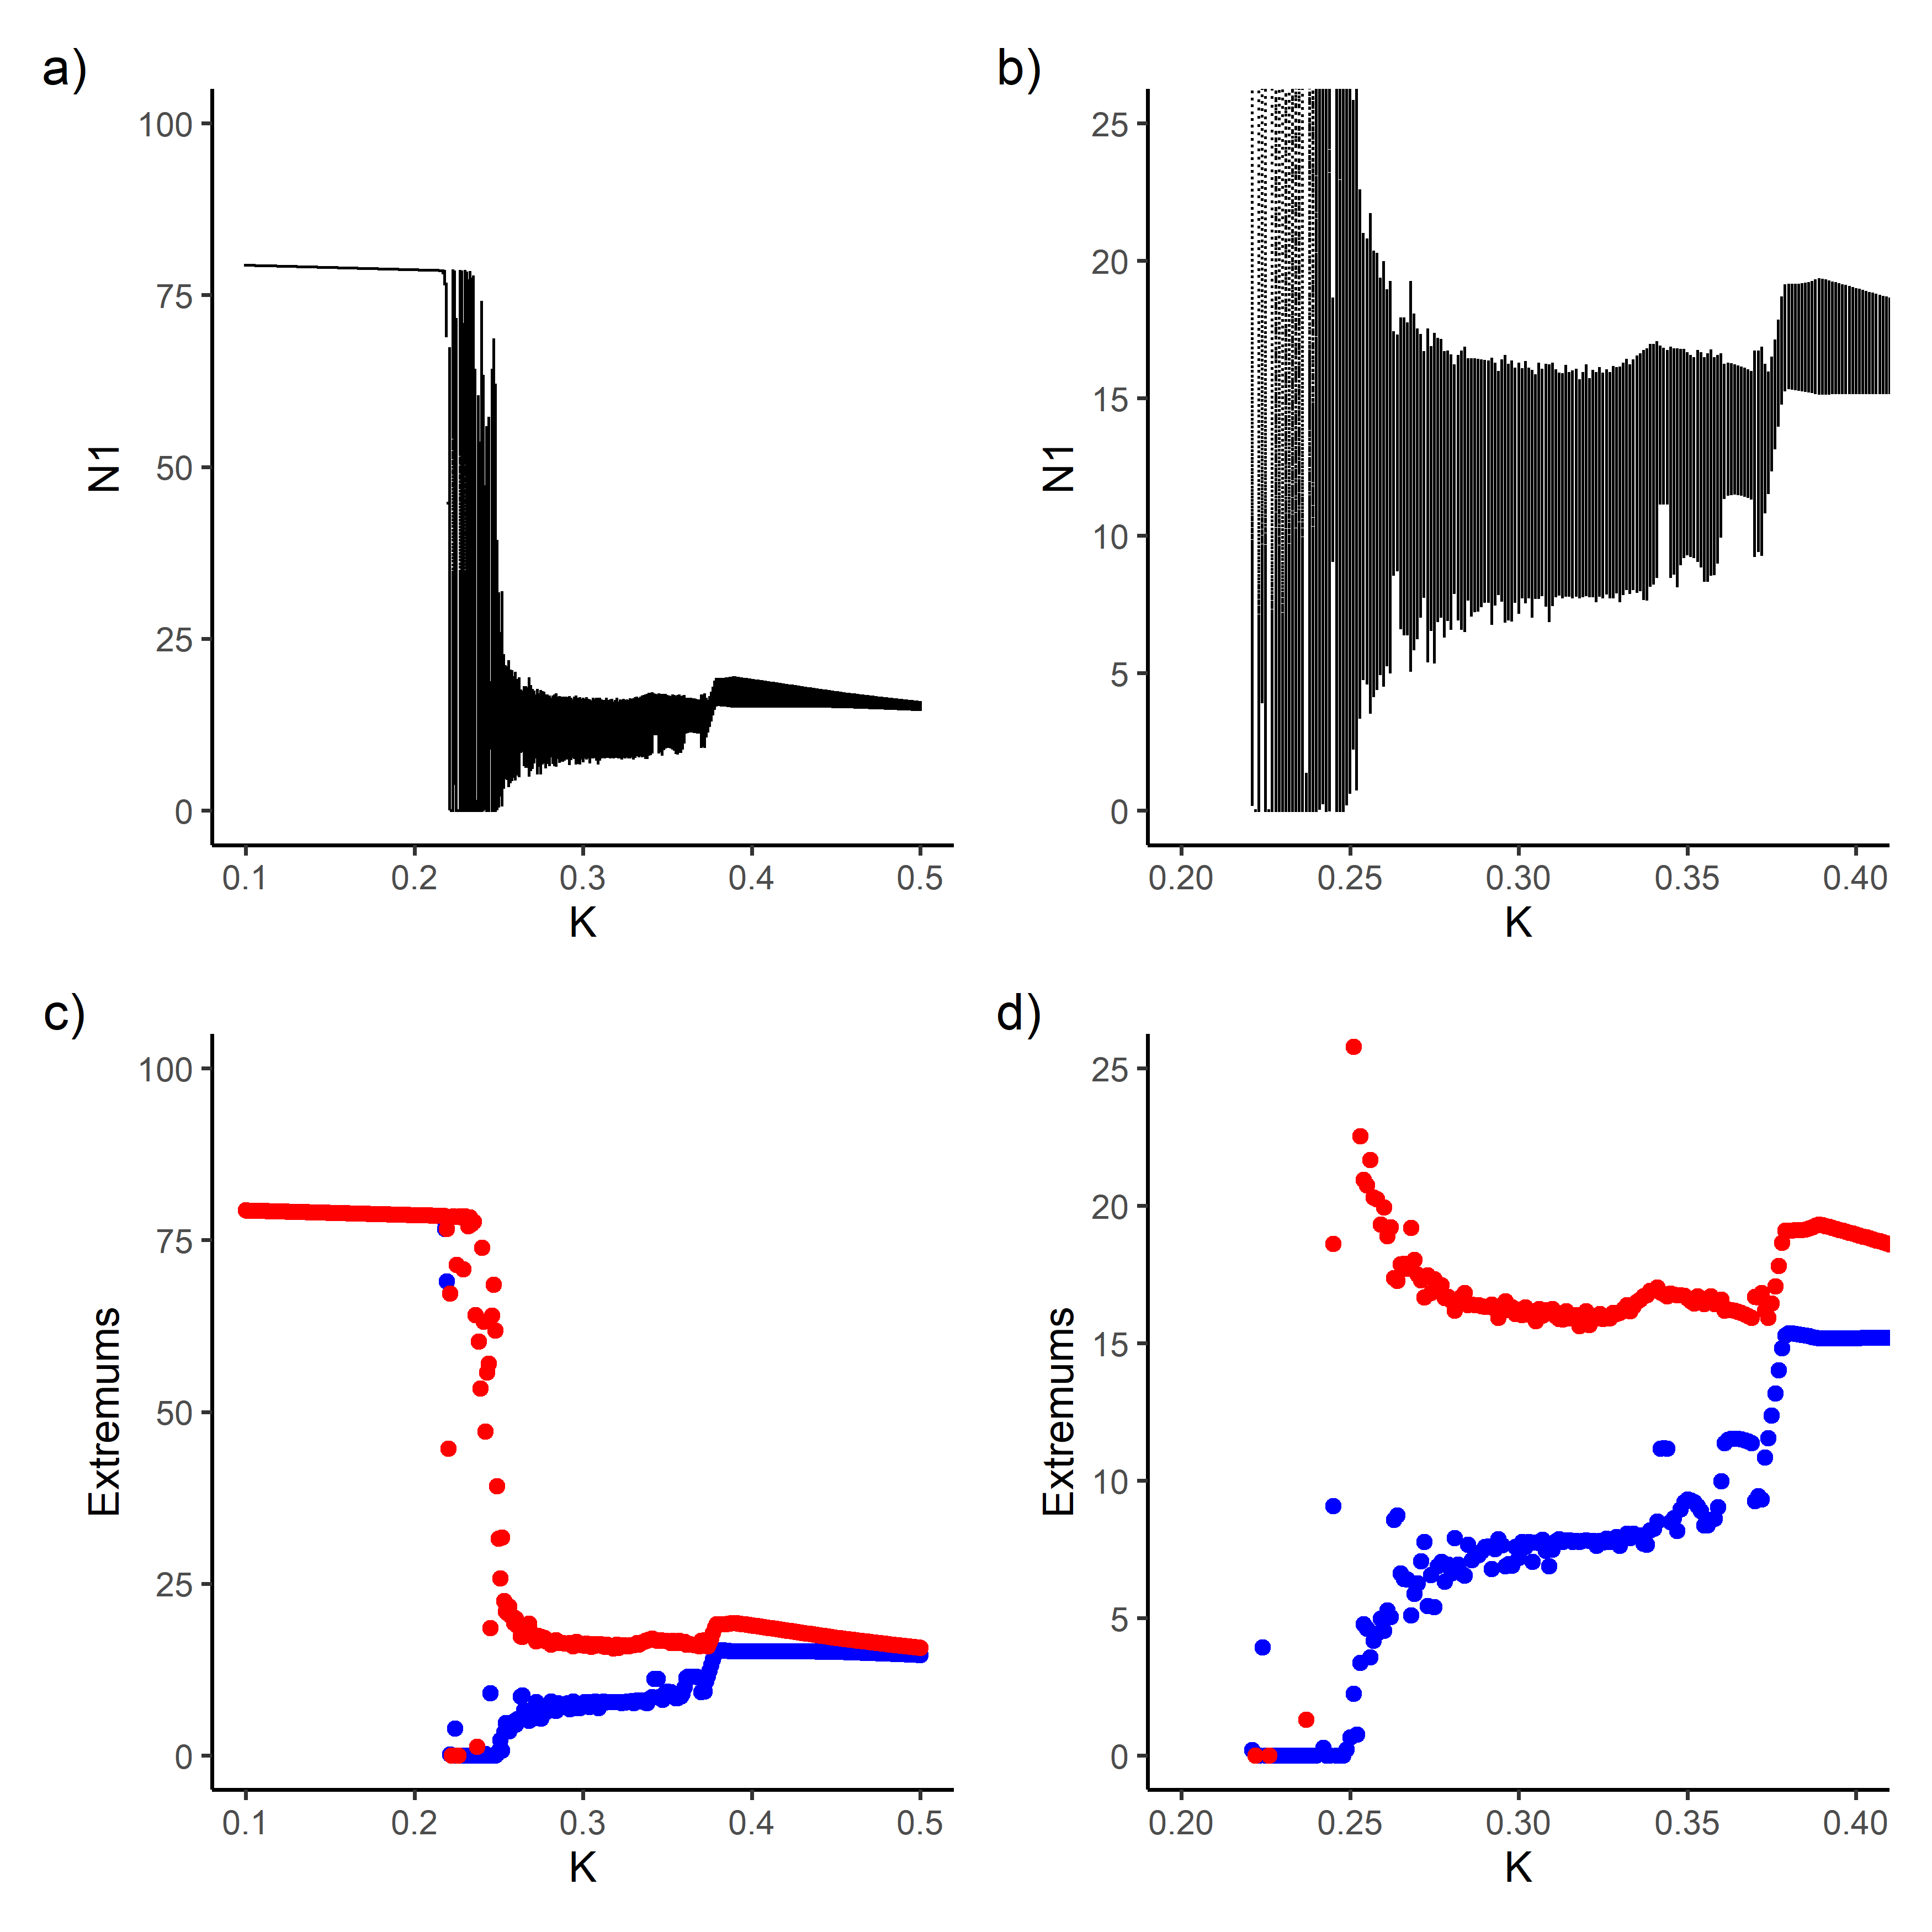
\includegraphics[width=1\textwidth]{../Code/Figures/Figure_3.png}
  \caption{Bifurcation diagram, for five species competing for five ressources. a) Show all of the vallues of species 1, plotted during the period from t=2,000 to t=4,000 days, as a function of the half-saturation constant K41. Part of a) is magnified in b). c) show the local minima and maxima of species 1, plotted during the period from t= 2,000 to t=4,000 days, as a function of the half-saturation constant K41. Part of c) is magnified in d).}
  \label{figures:Fig3}
\end{center}
\end{figure}
The bifurcation diagram caption didn't seemed to correspond to the actual Figure, which seemed to display all of the points of the simulation between $t=2,000$ and $t=4,000$ rather that only de local extremums.\\
We have therefore chosen to draw thoses two options. 
\begin{figure}[H]
\begin{center} 
 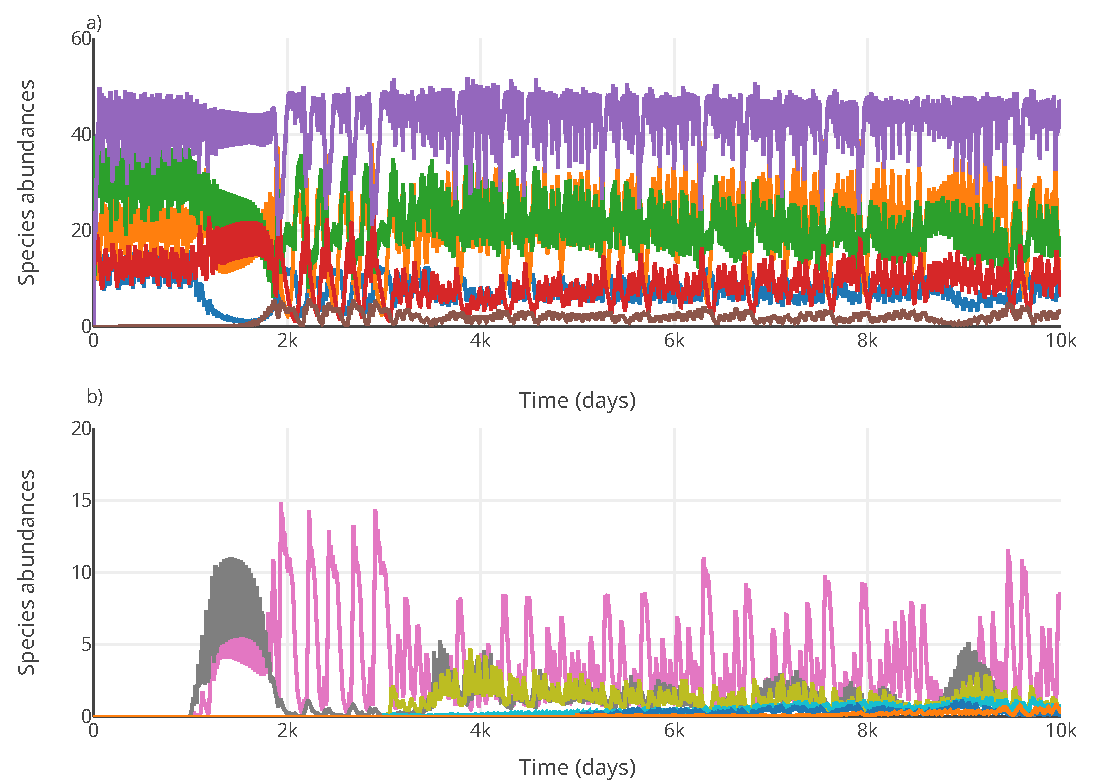
\includegraphics[width=0.86\textwidth]{../Code/Figures/Figure_4.pdf}
  \caption{Competitive chaos and the coexistence of 12 species on five resources. a),The abundances of species 1-6; b), the abundances of species 7-12}
  \label{figures:Fig4}
\end{center}
  \end{figure}
In order to conduct the experiment proposed earlier, the method used to plot the fourth Figure has been reused. The two experiment were conducted 400 times each, with as many different parameter sets : the $r_i$ were drawn according to a truncated normal distribution. The mean was $\mu=1$ and the variance was $\sigma=0.1$. The distribution was truncated using $\mu\pm3\sigma$,in other words between $0.7$ and $1.3$.\\
\\
For the first experiment, introducing species one after the other as in the original simulation, the following statistics, displaying the frequencies (expressed in \%) of the number of species present at the end of the simulation could be obtained : (A species has been considered present if $N_i > 0.001$ at the end of the simulation )\\
% latex table generated in R 4.2.1 by xtable 1.8-4 package
% Fri Jul 22 17:21:52 2022
\begin{table}[ht]
\centering
\begin{tabular}{rrrrrrrr}
  \hline
 & 0 species & 1 species & 2 species & 3 species & 4 species & 5 species & 6 species \\ 
  \hline
Probability & 0.00 & 13.68 & 26.56 & 35.01 & 11.27 & 8.85 & 4.02 \\ 
   \hline
\end{tabular}
\end{table}

% latex table generated in R 4.2.1 by xtable 1.8-4 package
% Fri Jul 22 17:21:52 2022
\begin{table}[ht]
\centering
\begin{tabular}{rrrrrrrr}
  \hline
 & 7 species & 8 species & 9 species & 10 species & 11 species & 12 species & Supersaturated \\ 
  \hline
Probability & 0.60 & 0.00 & 0.00 & 0.00 & 0.00 & 0.00 & 4.63 \\ 
   \hline
\end{tabular}
\end{table}

\\
This simulation shows that the subsitance of more than five species and more is very unlikely and so is the supersaturated coexitance in the parameter space.\\
\\
The pattern of extinction an its interaction with the sequential introduction of species is descirbed in the following Figure \ref{figures:Figexp1}, note that the subfigure 1) represent the original results with $r_i=1 ~\forall i$ : 
\begin{figure}[H]
\begin{center} 
 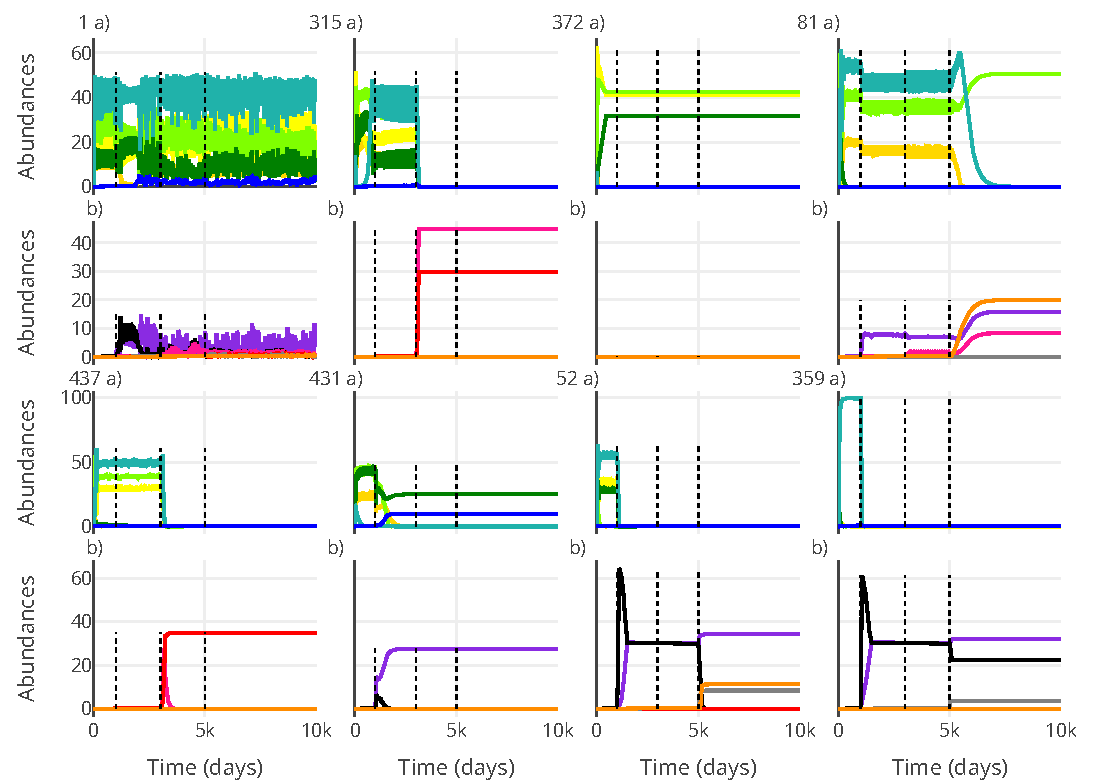
\includegraphics[width=1\textwidth]{../Code/Figures/Figure_exp1.pdf}
  \caption{Visualisation of 8 different simulations of competitive chaos and coexistance of 12 species on five ressources, following the Figure 4 method exept that $r_i$ was randomly for each of the species. Except the first one, the simulations illustrated were randomly picked among the 500 of the experience. a),The abundances of species 1-6 ; b), the abundances of species 7-12}
  \label{figures:Figexp1}
\end{center}
\end{figure}
We observe contrasted stationary endpoints, possibly with some oscillations or chaos during the invasion process. As shown in Figure\ref{figures:Tableexp1}, however, most species do not persist.\\
It is also noticable that the 5 species on 5 ressources (before the first invasion at $t=1,000$) is sometimes already unstable.\\
\\
For the second experiment, introducing all species at the same time, the following statistics could be obtained, displaying the frequencies (expressed in \%) of the number of species present at the end of the simulation : (A species has been considered present if $N_i > 0.001$ at the end of the simulation) \\
% latex table generated in R 4.2.1 by xtable 1.8-4 package
% Fri Jul 22 17:21:49 2022
\begin{table}[ht]
\centering
\begin{tabular}{rrrrrrrr}
  \hline
Extant species & 0 & 1 & 2 & 3 & 4 & 5 & 6 \\ 
  \hline
Probability & 0.00 & 36.40 & 41.40 & 5.00 & 10.00 & 6.00 & 1.20 \\ 
   \hline
\end{tabular}
\end{table}

% latex table generated in R 4.2.1 by xtable 1.8-4 package
% Fri Jul 22 17:21:49 2022
\begin{table}[ht]
\centering
\begin{tabular}{rrrrrrrr}
  \hline
 & 7 species & 8 species & 9 species & 10 species & 11 species & 12 species & Supersaturated \\ 
  \hline
Probability & 0.00 & 0.00 & 0.00 & 0.00 & 0.00 & 0.00 & 1.20 \\ 
   \hline
\end{tabular}
\end{table}

\\
This simulation shows that the subsitance of five species and more is very unlikely and the supersaturated coexistance very rare in the parameter space.\\
\\
The pattern of extinction an its interaction with the introduction of all of the species at the same time is descirbed in following Figure \ref{figures:Figexp2}, note that the subfigure 1) represent the original results with $r_i=1 ~\forall i$ : 
\begin{figure}[H]
\begin{center} 
 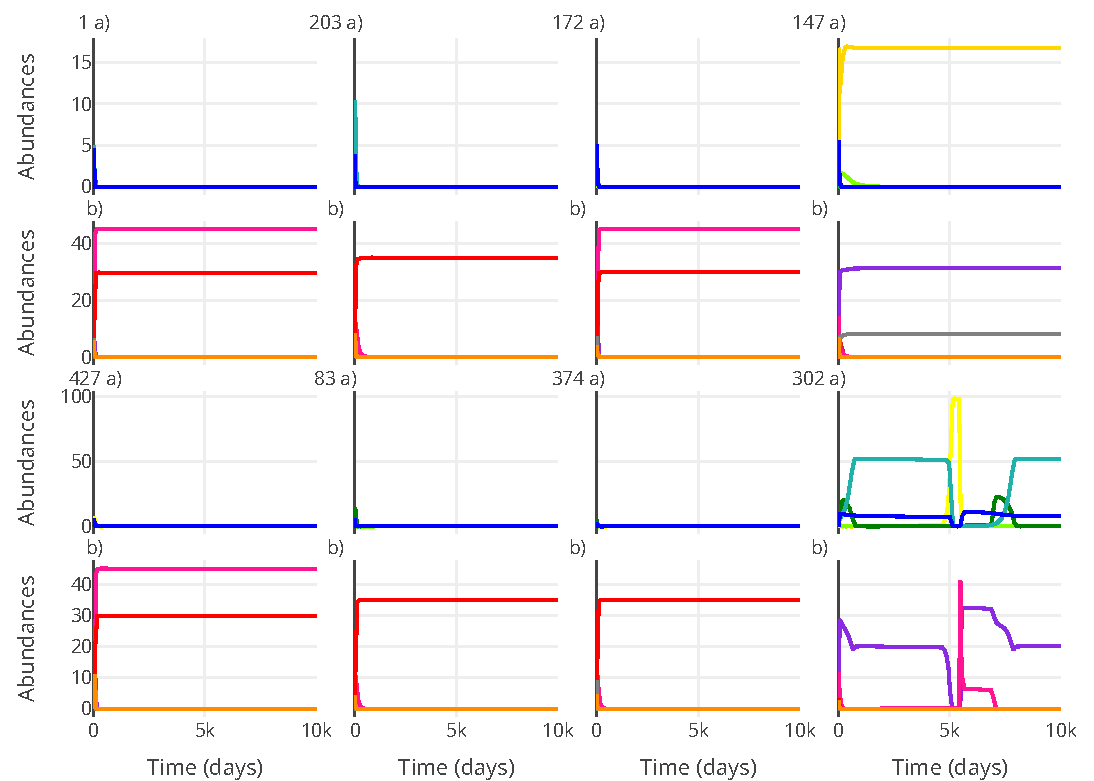
\includegraphics[width=1\textwidth]{../Code/Figures/Figure_exp2.pdf}
  \caption{Visualisation of 8 different simulations of competitive chaos and coexistance of 12 species on five ressources, following the Figure 4 method exept that $r_i$ was randomly for each of the species and all species were introduced at the same time. Except the first one, the simulations illustrated were randomly picked among the 500 of the experience. a),The abundances of species 1-6; b). the abundances of species 7-12}
  \label{figures:Figexp2}
\end{center}
  \end{figure}
As for the first experiment we observed either stationnary endpoints or oscillation but with even less persistent species as shown in Figure\ref{figures:Tableexp2}.
\section{Discussion}
We were able to successfully replicate the Figures of the original paper.\\ 
\\
Figure 4 shows minor differences arguably due to different integrations during the resolution.\\
\\
The experiments showed that slightly changing the $r_i$ parameter almost always prevents the coexistence of 12 species on five ressources and mostly prevents a supersaturated coexistance. This is true when introducing species sequentially as in the original paper as well as all at once. \\
\\
Those results corroborate the analisys of Schippers et al.\supercite{2008:Schippers} that supersaturated ceoexistence using chaos or oscillations are really unlikely in parameter space and requieres a really precise -in addition to being uncommon- parametrization. Our results are therefore consistent with their conclusion that the claim of solving the paradox of plankton might be premature.


